\documentclass[a4paper]{article}
\usepackage{amsmath}
\usepackage[english]{babel}
\usepackage{float}
\usepackage{graphicx}
\usepackage{hyperref}
\usepackage[utf8]{inputenc}
\usepackage{listings}
\usepackage{xcolor}

\usepackage{amsmath, amssymb, amsfonts, amsthm, mathtools} %doing math
\usepackage{algorithmicx, algpseudocode}

\newcommand{\summ}{\frac{1}{N}\sum_{i=1}^{N}}
\newcommand{\bw}{\mathbf{w}}
\newcommand{\bx}{\mathbf{x}}
\newcommand{\lra}{\Leftrightarrow}
\newcommand{\1}{\mathbbm{1}}
\newcommand{\E}{\mathbbm{E}}
\newcommand{\Prob}{\mathbb{P}} 
\newcommand{\itt}{\intertext}

% Sensible defaults for lstlistings
\lstset{
  basicstyle=\footnotesize\ttfamily,
  belowcaptionskip=1\baselineskip,
  breaklines=true,
  commentstyle=\bfseries\color{purple!40!black}
  frame=L,
  identifierstyle=\color{blue},
  keywordstyle=\bfseries\color{green!40!black},
  language=python,
  showstringspaces=false,
  stringstyle=\color{orange},
  xleftmargin=\parindent,
}

\title{\vspace{-5cm} Assignment 2}
\author{Silvan Robert Adrian - zlp432}

\begin{document}
\maketitle

% Usually unnecessary, but this simplifies grading for us TAs
\tableofcontents

\section{Illustration of Hoeffding's Inequality}
\subsection{Plotting Hoeffding}

I added the hoeffding bound to the following plot, which now includes all of the bounds including the empirical frequency.

To calculate the hoeffding bound I used $e^{-2 * n * (\epsilon^2)}$, from which I ended up on the following plot of the bound (including the other plots from assignment 1):

\begin{figure}[hbt!]
	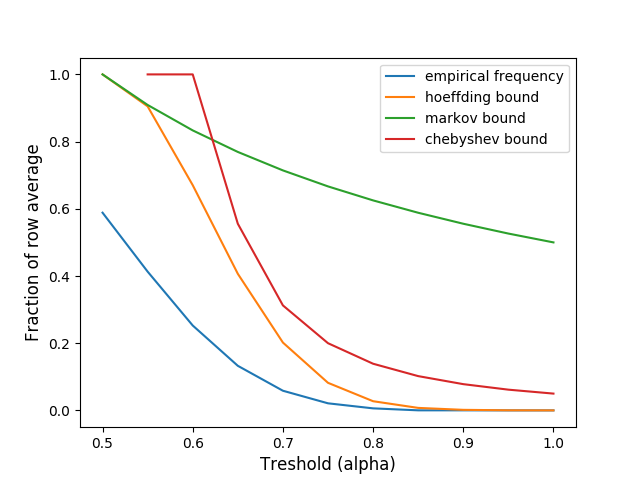
\includegraphics[width=\textwidth]{code/ex1}
	\caption{Plot with all bounds + the empirical frequency}
\end{figure}

\subsection{Compare}
Hoeffding bound overlaps at the beginning with markov but then fastly decreases, even faster then chebyshev which we compared in the first assignment already.
We also can discover that hoeffding gets better with a higher threshold, even better then chebyshev.

\subsection{Exact probability}
From Assignment 1 we have the following probabilities:
So before we got the probability for $\alpha = 0.95$: $\Pr\left[\frac 1 {20} \sum_{i=1}^{20} X_i \geq 0.95 \right] = \frac{21}{1024} \approx 0.0205078125$\\
and for $\alpha = 1$: $\Pr\left[\frac 1 {20} \sum_{i=1}^{20} X_i \geq 1 \right] = \frac 1 {1024} \approx 0.0009765625$

With hoeffding we just need to calculate it by using $e^{-2 * n * (\epsilon^2)}$, for that I directly used my programmed function in python:\\
then we get for $\alpha = 0.95$: $hoeffding(0.5,0.95,20) \approx 0.0003035391380788673$\\
and for $\alpha = 1$: $hoeffding(0.5,1,20) \approx 4.5399929762484854e-05$.\\
So the probabilities lay quite near to each other. Which also gets clear from the plot above, so that hoeffding lands is very near to the exact probability.
Which means for us the hoeffding estimation is very near the exact probability, so outputs quite good results in estimating the probabilities here.

\section{The effect of scale (range) and normalisation of random variables in
Hoeffding's inequality}
Let all the assumptions of \textbf{corollary 2.5} be true for some random variables $X_1, ..., X_n$. Set $a_i = 0$ and $b_i=1$ for all $i \in \{1, ..., n\}$. 
From \textbf{corollary 2.5} and our definition of $a_i$ and $b_i$, we now have it that all assumptions of \textbf{theorem 2.3} are true for $X_1, ..., X_n$. 
We can therefore use \textbf{theorem 2.3} to conclude that for all $\epsilon >0$.\\\\
From \textbf{theorem 2.3} we have:
\begin{align}
\mathbb{P}\left\{ \sum_{i=1}^n X_i - \mathbb{E}\left[ \sum_{i=1}^n X_i \right] \geq \epsilon \right\} \leq e^{-2 \epsilon^2 / \sum_{i=1}^n (b_i - a_i)^2}
\end{align}
and
\begin{align}
\mathbb{P}\left\{ \sum_{i=1}^n X_i - \mathbb{E}\left[ \sum_{i=1}^n X_i \right] \leq - \epsilon \right\} \leq e^{-2 \epsilon^2 / \sum_{i=1}^n (b_i - a_i)^2}
\end{align}
%% use corollary 2.5, which states
The \textbf{corollary 2.5} states $\mathbb{E}(X_i) = \mu$ for all $i \in \{1, ..., n\}$, then we know that:
\begin{align}
\mathbb{E}\left[ \sum_{i=1}^n X_i \right] = n\mu 
\end{align}
Since $b_i - a_i = 1$ for all $i \in \{1, ..., n\}$, we also know that:
\begin{align}
\sum_{i=1}^n (b_i - a_i)^2 = n 
\end{align}
%% move into the above equalities for both probabilities
By using all the above learned we get for all $\epsilon > 0$ following:
\begin{align}
\mathbb{P}\left\{ \sum_{i=1}^n X_i - n\mu \geq \varepsilon \right\} \leq e^{- 2 \frac{\varepsilon^2}{n} } = e^{- 2n \left( \frac{ \varepsilon}{n} \right)^2 }
\end{align}
and
\begin{align}
\mathbb{P}\left\{ \sum_{i=1}^n X_i - n\mu \leq -\varepsilon \right\} \leq e^{- 2 \frac{\varepsilon^2}{n} } = e^{- 2n \left( \frac{ \varepsilon}{n} \right)^2 }
\end{align}
By putting it then into the \textbf{corollary 2.5}, we see that for all $\epsilon > 0$ follows that:
\begin{align}
\mathbb{P}\left\{\frac{1}{n} \sum_{i=1}^n X_i - \mu \geq \frac{\varepsilon}{n} \right\} \leq = e^{- 2n \left( \frac{ \varepsilon}{n} \right)^2 }
\end{align}
and
\begin{align}
\mathbb{P}\left\{\frac{1}{n} \sum_{i=1}^n X_i - \mu \leq- \frac{\varepsilon}{n} \right\} \leq = e^{- 2n \left( \frac{ \varepsilon}{n} \right)^2 }
\end{align}
Then it's clear that we can redefine the $\epsilon$ as $\tilde{\epsilon} = \frac{\epsilon}{n} > 0$, so that we can conclude that for all $\tilde{\epsilon}>0$:
\begin{align}
\mathbb{P}\left\{\frac{1}{n} \sum_{i=1}^n X_i - \mu \geq \tilde{\epsilon} \right\} \leq = e^{- 2n \tilde{\epsilon}^2 }
\end{align}
and
\begin{align}
\mathbb{P}\left\{\frac{1}{n} \sum_{i=1}^n X_i - \mu \leq - \tilde{\epsilon} \right\} \leq = e^{- 2n \tilde{\epsilon}^2 }
\end{align}
%% prove finished
So we have proven that \textbf{corollary 2.5} follows from \textbf{theorem 2.3}.

\section{A Very Practical Question}
\subsection{markov}
-
\subsection{}

\section{Probability in Practice (``The Airline Question'')}
%
%% Exercise 3
%
\subsection{Question 1}
We assume that the probability of each passenger showing up is 0.95 (since probability of not showing up is 0.05), and that the event of a passenger showing up is independent (which is the case according to the description).
Which implies $P[passenger showin gup] = 0.95$, from which we can calculate

\begin{align}
\left( \frac{95}{100} \right)^{100} = 0.00592... \approx 0.006	
\end{align}
So for 6 out of 1000 flights there might show up too many passengers, so the plane won't have enough seats left for all passengers in those cases.

\subsection{Question 2}
We have given the following Events:
\begin{enumerate}
	\item 95\% of passengers showing up out of 10000, where each passenger shows up with the probability $p$
	\item 100 passengers show up each with the probability of $p$ (everybody shows up)
\end{enumerate}

From those 2 Events we get the probability that 9500 of 10000 persons getting on their plane and all 100 passengers arriving to one given airplane (overbooking).
With this information we use the hoeffding bound for the probability of 9500 arriving to a plane.
When this bound is found we then can multiply it by the probability that a plane gets overbooked ($p^{100}$).
Then I can solve for $p$ and find the bound.
 
\begin{align}
	&\Prob \left( \sum_{i=1}^{10000} X_{i} \geq 9500 \right) \\
	= &\Prob \left( \sum_{i=1}^{10000} X_{i} - 10000\cdot p \geq 9500 - 10000\cdot p \right)  \\
	\leq &e^{-2(10000(0.95-p))^2 / \sum_{i=1}^{10000}(b_{i} - a_{i})^{2}} \\
	=& \leq e^{-2(10000(0.95-p))^2 / \sum_{i=1}^{10000}(0 - 1)^{2}} \\
	=&  \leq e^{-2(10000(0.95-p))^2 / \sum_{i=1}^{10000}1} \\
	=&  \leq e^{-2(10000(0.95-p))^2 / 10000}
\intertext{Now using the expression for the probability (bound) of all people arriving to the plane $p^{100}$ the probability can be bound:}
	&p^{100}\cdot e^{-2(10000(0.95-p))^2 / \sum_{i=1}^{10000}1}  = 0.006797
\end{align}
 
When we solve the equation numerically we will find $p=0.9526$.
 The figure below (figure \ref{fig:ex3} shows the corresponding bound given probability $p$.

\begin{figure}[!htb]
	\center
	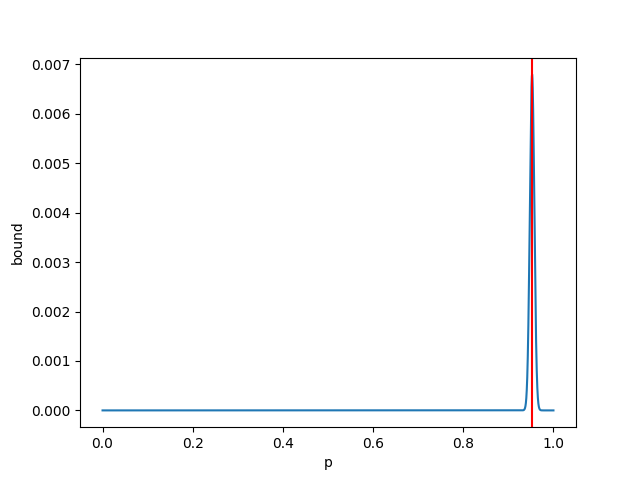
\includegraphics[width=\textwidth]{code/ex3}
	\caption{showing the bound to the corresponding probability, while the red line is the worst case p}
	\label{fig:ex3}
\end{figure}

\section{Logistic Regression}
\subsection{Cross entropy error measure}


We start by defining $X$ to be a sample space and $Y$ be the label space of \{-1,1\}.
We want to learn the conditional probability $P(y|x)$ for $y \in {-1,1}$ and all $x \in X$.
But we have to be able to parametrize $P(y|x)$ by $w$, which we choose from a parameter space so that $w \in W$.
This way we get the value of $P_w(y|x)$ for $y \in -1,1$ and all $x \in X$.

Now we need a function to choose some parameter $\hat{w} \in W$ and therefore a corresponding distribution $P_{\hat{w}}(y|x)$ as well.
The only information on which we can make these assumptions is the labeled sample $S = \{(x_1,y_1),...,(x_N,y_N)\}$. 

I use the maximum likelihood function for that with the parameter $w$ as described above with the given sample $S$:
\begin{align}
L_S(w) = \prod_{(x_n,y_n)\in \mathcal{S}}  P_w(y_n|x_n)
= \prod_{n=1}^N P_w(y_n|x_n)
\end{align}
and then saying that we should choose $\hat{w} \in \mathcal{W}$ such that $L_\mathcal{S}$ is maximized.

Since the function $-\ln$ is monotonically decreasing, this strategy is equivalent\footnote{I define two strategies to be equivalent, if and only if they end up choosing the same $\hat{w}$ for all possible samples $S = \{(x_1,y_1),...,(x_N,y_N)\}$.} to choosing $\hat{w} \in \mathcal{W}$ such that the function
\begin{align}
f_S(w) = -\ln \left( \prod_{n=1}^N P_w(y_n|x_n) \right) = \sum_{n=1}^N \left( - \ln P_w(y_n|x_n) \right)
\end{align}
is minimized. 

Since $y \in \{-1,1\}$, then we can write $P_w(y|x)$ as
\begin{align}
P_w(y|x)  = \\ 
[[y = 1]] P_w(y = 1|x) + [[y = 1]] P_w(y = -1|x) = \\ 
[[y = 1]] h_w(x) + [[y = 1]] (1 - h_w(x))
\end{align}
where we simply have defined $h_w(x) = P(y = 1 | x)$. We therefore have that
\begin{align}
- \ln P_w(y_n|x_n) = \\ 
-\ln ([[y = 1]] h_w(x) + [[y = -1]] (1 - h_w(x))) = \\ 
[[y = 1]](-\ln (h_w(x)) + [[y = -1]](-\ln (1 - h_w(x))) = \\ 
[[y = 1]]\left(\ln \left( \frac{1}{h_w(x)}\right)\right) + [[y = -1]]\left(\ln \left( \frac{1}{1 - h_w(x)}\right)\right)
\end{align}

By line (2) and line (6-9), we now get that
\begin{align}
f_S(w) = \sum_{n=1}^N \left[ [[y_n = 1]]\left(\ln \left( \frac{1}{h_w(x_n)}\right)\right) + [[y_n = -1]]\left(\ln \left( \frac{1}{1 - h_w(x_n)}\right)\right) \right]
\end{align}
As I have already said, we will end up with the same $\hat{w}$ for a given sample $S$, if we minimize $f_S(w)$ as if we maximize $L_S(w)$. If we had started by saying that we would like to estimate the probability $h_w(x) = P_w(y = 1|x)$ by choosing $\hat{w}$ such that we minimize the error function $f_S(w)$ defined as in line (10), we would have ended up with the same estimates of $P(y|x)$ for $y \in \{-1,1\}$ and $x\in \mathcal{X}$, as if we have used the maximum likelihood method. These two strategies are therefore equivalent.

If we now focus on logistic regression and set $h_w(x) = \Theta(w^T x) = \frac{e^{w^Tx}}{1 + e^{w^Tx}}$, we know from the book that $1 - h_w(x) = h_w(-x)$, which means that
\begin{align}
f_S(w) = \sum_{n=1}^N \left[ [[y_n = 1]]\left(\ln \left( \frac{1}{h_w(x_n)}\right)\right) + [[y_n = -1]]\left(\ln \left( \frac{1}{h_w(-x_n)}\right)\right) \right] = \\
 \sum_{n=1}^N  \ln \left( \frac{1}{h_w(y_nx_n)}\right)  = \sum_{n=1}^N  \ln \left( \frac{1}{\frac{e^{y_nw^Tx}}{1 + e^{y_ nw^Tx}}}\right)  = \sum_{n=1}^N  \ln \left( \frac{1 + e^{y_ nw^Tx}}{e^{y_ nw^Tx}}\right)  = \\
 \sum_{n=1}^N  \ln \left( 1 +e^{-y_ nw^Tx}\right)
\end{align}
Minimizing this function gives the same $w$ as minimizing:
\begin{align}
\frac{1}{N}f_S(w) = \frac{1}{N} \sum_{n=1}^N  \ln \left( 1 +e^{-y_ nw^Tx}\right)
\end{align}
This is exactly the function that the book says in statement (3.9) that we should minimize, when we search for the weights in logistic regression.


\subsection{Logistic regression loss gradient}

In the algorithm for logistic regression, we determine the parameter $w \in \mathbb{R}^m$ in our final hypothesis
\begin{align}
h_w(x) = P_w(y = 1|x) = \frac{e^{w^Tx}}{1 + e^{w^Tx}}
\end{align}
using a given labeled sample $S = \{(x_1,y_1),...,(x_N,y_N)\}$ by minizing the function
\begin{align}
E_{in}(w) = \frac{1}{N} \sum_{n=1}^N \ln(1 + e^{-y_n w^T x_n})
\end{align}
We use gradient descent to do this, which means we have to find the loss gradient $\nabla E_{in}(w)$. We can use matrix calculus to to differentiate $E_{in}$
\begin{align}
D_w (E_{in}(w)) = D_w\left( \frac{1}{N} \sum_{n=1}^N \ln(1 + e^{-y_n w^T x_n}) \right) = \\ 
 \frac{1}{N} \sum_{n=1}^N D_w \left( \ln(1 + e^{-y_n w^T x_n}) \right). 
\end{align}
Let us now focus on the inside of the sum
\begin{align}
D_w \left( \ln(1 + e^{-y_n w^T x_n}) \right) = \frac{D_w ( 1 + e^{-y_n w^T x_n})}{1 + e^{-y_n w^T x_n}} = \\ 
\frac{D_w (e^{-y_n w^T x_n})}{1 + e^{-y_n w^T x_n}} =
\frac{e^{-y_n w^T x_n} D_w(-y_nw^Tx)}{1 + e^{-y_n w^T x_n}} = \\ 
-y_n x_n \frac{e^{-y_n w^T x_n}}{1 + e^{-y_n w^T x_n}} = -y_n x_n \Theta(-y_n w^T x_n)
\end{align}
Line (13-14) and line (15-17) now gives us that
\begin{align}
D_w (E_{in}(w)) =  \frac{1}{N} \sum_{n=1}^N D_w \left( \ln(1 + e^{-y_n w^T x_n}) \right) =
\frac{1}{N} \sum_{n=1}^N  -y_n x_n \Theta(-y_n w^T x_n) 
\end{align}



\subsection{Logistic regression implementation}


\subsection{Iris Flower Data}


\end{document}

